\chapter{Implementacija i korisničko sučelje}
		
		
		\section{Korištene tehnologije i alati}
		
			\textbf{\textit{dio 2. revizije}}
	
			Komunikacija članova tima realizirana je aplikacijom Discord\footnote{https://discord.com/}. Dokumentacija je pisana u alatu TEXstudio\footnote{https://www.texstudio.org//}, a UML dijagrami crtani su alatom Astah\footnote{https://astah.net/}. Sustav za upravljanje izvornim kodom je Git\footnote{https://git-scm.com/}, a udaljeni repozitorij projekta dostupan je na web platformi GitLab\footnote{https://gitlab.com/}. Kao razvojno okruženje za frontend koristio se Visual Studio Code\footnote{https://code.visualstudio.com/} dok su se  za backend koristili su se IntelliJ IDEA\footnote{https://www.jetbrains.com/idea/} i Eclipse\footnote{https://www.eclipse.org/}. Za izradu aplikacije korištene su tehnologije Spring Boot\footnote{https://spring.io/projects/spring-boot} za backend te React\footnote{https://reactjs.org/} za frontend. Tehnologija Spring Boot zahtjeva programiranje u Javi\footnote{https://www.java.com/en/}, a tehnologija React programiranja u JavaScriptu\footnote{https://www.javascript.com/}. Sustav baze podataka ove aplikacije je PostgreSQL\footnote{https://www.postgresql.org/}. Još treba napisati u čemu smo testirali aplikaciju, uključujući korištene biblioteke.
%			 \textit{
%			 	Detaljno navesti sve tehnologije i alate koji su primijenjeni pri izradi dokumentacije i aplikacije. Ukratko ih opisati, te navesti njihovo značenje i mjesto primjene. Za svaki navedeni alat i tehnologiju je potrebno \textbf{navesti internet poveznicu} gdje se mogu preuzeti ili više saznati o njima}.
			
			
			\eject 
		
	
		\section{Ispitivanje programskog rješenja}
			
			\begin{comment}
			\textbf{\textit{dio 2. revizije}}\\
			 \textit{U ovom poglavlju je potrebno opisati provedbu ispitivanja implementiranih funkcionalnosti na razini komponenti i na razini cijelog sustava s prikazom odabranih ispitnih slučajeva. Studenti trebaju ispitati temeljnu funkcionalnost i rubne uvjete.}
			\end{comment}
			
			\subsection{Ispitivanje komponenti}
			Kako bi se uvjerili u ispravnost pojedinih klasa i metoda proveli smo ispitivanje jedinica (engl. unit testing) nad razredima koji implementiraju temeljne funkcionalnosti. Testove smo napisali tako da ispituju redovne slučajeve, ali i rubne slučajeve.
			Koristili smo javin open source framework za testiranje JUnit.\\
			
			\noindent\textbf{Ispitni slučaj 1: traženje korisnika po korisničkom imenu}\\
			Sljedeća dva testa provjeravaju funkcionalnosti klase userService.
			Klasa userService pruža metodu za dohvat korisnika na temelju njegovog korisničkog imena.
			Tu metodu smo testirali sa validnim korisničkim imenom "athlete" u metodi testFindGoodUsername te sa imenom nepostojećeg korisnika u metodi
			 testFindBadUsername.
			 
			 \begin{lstlisting}[language=Java,caption={findByUsername},label=DescriptiveLabel]
@Test
void testFindGoodUsername() {
  Optional < User > user = userService.findByUsername("athlete");
  assertThat(user.isPresent());
}

@Test
void testFindBadUsername() {
  Optional < User > user = userService.findByUsername("wrongUsername");
  assertThat(user.isEmpty());
}
			 \end{lstlisting}
		
			\noindent Rezultat izvođenja ispitnog slučaja: Ispit je uspješan.

				%tu dodat slike kad se runna JUnit test.
			
			
			\hfill\break
			\noindent\textbf{Ispitni slučaj 2: Dodavanje i spremanje korisnika.}\\
			Slijedećim testom provjerili smo funkcionalnosti stvaranja i dodavanja novog korisnika sportaša. Testirane metode također su dio klase userService.
			
			\begin{lstlisting}[language=Java,caption={testSaveAndFindUser},label=DescriptiveLabel]
@Test
void testSaveAndFindUser() {
  User user = new Athlete("newUsername", "newPassword", "e@mail.com", "name", "surname");
  userService.save(user);
  Optional < User > user1 = userService.findByUsername("newUsername");
  assertThat(user1.isPresent());
}

			\end{lstlisting}
			\noindent Izvođenje ispitanog slučaja: Ispit je uspješan.
			
			\hfill\break
			\noindent\textbf{Ispitni slučaj 3: Testiranje kontrolera za sportske događaje.}\\
		Naredna dva testa provjerava kontroler sportskih događaja,
		 odnosno klasu sportEventController. 
		U testu testSporteventControllerFindByGoodId() kreiramo http get request na /api/v1/sportevents/2   da bi provjerili dostupnost postojećeg sportskog eventa, sportskog eventa pod brojem 2.
			Analogno u metodi testSporteventControllerFindByBadId() pokušavamo dohvatiti nepostojeći sportski event, event koji ima is 2000.
			
			\begin{lstlisting}[language=Java,caption={testSporteventControllerFindById},label=DescriptiveLabel]
@Test
void testSporteventControllerFindByGoodId() throws Exception {
  this.mockMvc.perform(get("/api/v1/sportevents/2"))
              .andDo(print()).andExpect(status().isOk());
}

@Test
void testSporteventControllerFindByBadId() throws Exception {
  this.mockMvc.perform(get("/api/v1/sportevents/2000"))
              .andDo(print()).andExpect(status().isBadRequest());
}
			\end{lstlisting}
			\noindent Izvođenje ispitanog slučaja: Ispit je uspješan.
			
			\hfill\break
			\noindent\textbf{Ispitni slučaj 4: Testiranje kontrolera za sportske lokacije.}\\
			Na sličan način testirali smo i funkcionalnosti kontrolera za sportske lokacije odnosno klasu locationController.
			
			\begin{lstlisting}[language=Java,caption={testLocationControllerFindById},label=DescriptiveLabel]	
	@Test
	void testLocationControllerFindByGoodId() throws Exception{
		this.mockMvc.perform(get("/api/v1/locations/1")).andDo(print()).andExpect(status().isOk());
	}

	@Test
	void testLocationControllerFindByBadId() throws Exception{
		this.mockMvc.perform(get("/api/v1/locations/1000")).andDo(print()).andExpect(status().isBadRequest());
	}

	        \end{lstlisting}
			\noindent Izvođenje ispitanog slučaja: Ispit je uspješan.
		\hfill\break
	
	Ranije navedene testove pokrenuli smo u razvojnom okruženju Eclipse IDE. Rezultati testova vidljivi su na slici ispod.		
			
	\begin{figure}[H]
			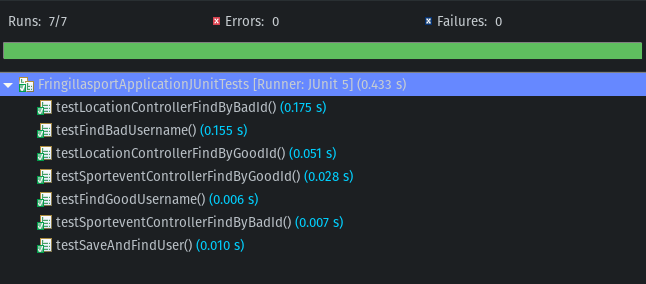
\includegraphics[width=1\linewidth]{slike/JUnitTestovi.PNG}
			\centering
			\caption{rezultati JUnit testova}
			\label{fig:promjene}
		\end{figure}			
			
			\subsection{Ispitivanje sustava}
			
			 Proveli smo ispitivanje sustava koristeći radni okvir Selenium\footnote{\url{https://www.seleniumhq.org/}}.U nastavku ispitujemo 4 ispitna slučaja u kojima testiramo redovne slučajeve, rubne uvjete te namjerno korištenje aplikacije na neočekivani način kako bi se vidjelo na koji način sustav reagira.%Ispitni slučaj se treba sastojati od ulaza (npr. korisničko ime i lozinka), očekivanog izlaza ili rezultata, koraka ispitivanja i dobivenog izlaza ili rezultata.\\ 
			 
			 Za ispitivanje koristili smo alat \textbf{Selenium WebDriver} te programski jezik javu.
			 
			 
			 \hfill\break
			 \noindent\textbf{Ispitni slučaj 1: Prijava u sustav}
			 
			 
			 Da bi korisnik koristio našu web aplikaciju mora se prijaviti u sustav sa već postoječim korisničim računom ili treba prvo napraviti registraciju pa zatim prijavu.
			 Slijedeći test testira prijavu na stranicu sa već postojećim korisničkim računom za sportaša. Nakon uspiješne prijave web aplikacija izbacuje iskočnu poruku koja prikazuje tekst "uspiješna prijava". Funkcionalnost je testirana u metodama testLoginGoodCreds() i testLoginBadCreds().
			 
			 
			 \hfill\break
			 \noindent\textbf{Ulaz:}
			 
			 \begin{packed_enum}
			 	
			 	\item Otvaranje početne stranice u web pregledniku
			 	\item Klik na gumb prijava
			 	\item Unos korisničkog imena
			 	\item Unos lozinke
			 	\item Klik na gumb prijava
			 	
			 	
			 	
			 \end{packed_enum}
			 
			 \noindent\textbf{Očekivani rezultat:}
			 
			 \begin{packed_enum}
			 	
			 	\item Otvorila se početna stranica
			 	\item Prikzala se stranica za prijavu
			 	\item Popunilo se polje za korinsičko ime i šifru
			 	\item Prikazuje se skočna poruka za uspješnu prijavu
			 	\item Prikazuje se profil korisnika
			 	
			 	
			 	
			 \end{packed_enum}
			 
			 \noindent\textbf{Rezultat:} Sva očekivanja su zadovoljena. Selenium test je prošao.
			 
			 
			 \begin{lstlisting}[language=Java,caption={testLoginGoodCreds},label=DescriptiveLabel]	
@Test
void testLoginGoodCreds() {

	System.setProperty("webdriver.chrome.driver", 
	"/Users/Luka/Applications/WebDriver/chromedriver");
	WebDriver driver = new ChromeDriver();

	driver.manage().timeouts().implicitlyWait(10, TimeUnit.SECONDS);
	driver.get("http://localhost:3000/prijava");

	WebElement element = driver.findElement(
	By.xpath("//*[@id=\"root\"]/div/div[2]/div[1]/form/div[1]/div[2]/input"));        
	element.sendKeys("athlete");

	element = driver.findElement(By.xpath(
	"//*[@id=\"root\"]/div/div[2]/div[1]/form/div[2]/div[2]/input"));
	element.sendKeys("athlete");

	driver.findElement(By.xpath(
	"//*[@id=\"root\"]/div/div[2]/div[1]/form/button")).click();

	WebDriverWait wait = new WebDriverWait(driver, 5);
	Alert alert = wait.until(ExpectedConditions.alertIsPresent());
	String alertCheck=alert.getText();
	boolean compRes= alertCheck.contains("Uspjesna");

	assertTrue(compRes);
	driver.quit();
}

			 \end{lstlisting}
			 
			 \hfill\break
			 \noindent\textbf{Ispitni slučaj 2: Prijava s krivim podacima}
		
		Analogni test za prijavu napravili smo i krivim korisničkim podatcima. Očekivani rezultat je poruka upozorenja sa tekstom "Pogreška"
		
			\hfill\break
			\noindent\textbf{Ulaz:}
			
			\begin{packed_enum}
				
				\item Otvaranje početne stranice u web pregledniku
			 	\item Klik na gumb prijava
			 	\item Unos nepostojećeg korisničkog imena
			 	\item Unos nepostojeće lozinke
			 	\item Klik na gumb prijava
				
			\end{packed_enum}
			
			\noindent\textbf{Očekivani rezultat:}
			
			\begin{packed_enum}
				
				\item Otvorila se početna stranica
			 	\item Prikzala se stranica za prijavu
			 	\item Popunilo se polje za korinsičko ime i šifru
			 	\item Prikazuje se skočna poruka za grešku prilikom prijave
				
			\end{packed_enum}
			
			\noindent\textbf{Rezultat:} Sva očekivanja su zadovoljena. Selenium test je prošao.
		
		\begin{lstlisting}[language=Java,caption={testLoginBadCreds},label=DescriptiveLabel]
@Test
void testLoginBadCreds() {
	System.setProperty("webdriver.chrome.driver",
 "/Users/Luka/Applications/WebDriver/chromedriver");
	WebDriver driver = new ChromeDriver();

	driver.manage().timeouts().implicitlyWait(10, TimeUnit.SECONDS);
	driver.get("http://localhost:3000/prijava");

	WebElement element = driver.findElement(By.xpath(
	"//*[@id=\"root\"]/div/div[2]/div[1]/form/div[1]/div[2]/input"));        
	element.sendKeys("wrongUsername");

	element = driver.findElement(By.xpath(
	"//*[@id=\"root\"]/div/div[2]/div[1]/form/div[2]/div[2]/input"));
	element.sendKeys("WrongPassword");

	driver.findElement(By.xpath(
	"//*[@id=\"root\"]/div/div[2]/div[1]/form/button")).click();

	WebDriverWait wait = new WebDriverWait(driver, 5);
	Alert alert = wait.until(ExpectedConditions.alertIsPresent());
	String alertCheck=alert.getText();
	boolean compRes= alertCheck.contains("Pogreska");

	assertTrue(compRes);
	driver.quit();
}

		\end{lstlisting}
		
		\hfill\break
		\noindent\textbf{Ispitni slučaj 3: Prijava na sportsko događanje}
		
		Aplikacija prijavljenim korisnicima nudi mogućnost da se se prijave na neko od nadolazećih sportskih događanja nakon čega sustav prikazje poruku "Uspješno".
		Tu funkcionalnost provjerili smo u klasi SeleniumApplyForEventTest metodom testApplyForEvent.
		
		\hfill\break
		\noindent\textbf{Ulaz:}
		
		\begin{packed_enum}
			
				\item Otvaranje početne stranice u web pregledniku
			 	\item Klik na gumb prijava
			 	\item Unos korisničkog imena
			 	\item Unos lozinke
			 	\item Klik na gumb prijava
			 	\item Klik na gumb karta sportskih okupljanja
			 	\item Klik na prvi event u prikazanoj listi sportskih okupljanja
			 	\item Klik na gumb prijava
			 	\item Klik na gumb za potvrdu prijave
			
		\end{packed_enum}
		
		\noindent\textbf{Očekivani rezultat:}
		
		\begin{packed_enum}
			
				\item Otvorila se početna stranica
			 	\item Prikzala se stranica za prijavu
			 	\item Popunilo se polje za korinsičko ime i šifru
			 	\item Prikazuje se skočna poruka za uspješnu prijavu
			 	\item Prikazuje se stranica s korisnikovim podacima
			 	\item Prikazuje se stranica s kartom i popisom sportskih ikupljanja
			 	\item Prikazuju se detalji o prvom sportskom eventu
			 	\item Prikazuje se skočna poruka za potvrdu prijave
			 	\item Pored sportskog događaja korisniku piše da je prijavljen na njega
			 	
				
				
		\end{packed_enum}
		
		\noindent\textbf{Rezultat:} Sva očekivanja su zadovoljena. Selenium test je prošao.
		
		\begin{lstlisting}[language=Java,caption={testApplyForEvent},label=DescriptiveLabel]
@Test
void testApplyForEvent() {

	System.setProperty("webdriver.chrome.driver",
 "/Users/Luka/Applications/WebDriver/chromedriver");
	WebDriver driver = new ChromeDriver();

	driver.manage().timeouts().implicitlyWait(10, TimeUnit.SECONDS);
	driver.get("http://localhost:3000/prijava");

	WebElement element = driver.findElement(By.xpath(
	"//*[@id=\"root\"]/div/div[2]/div[1]/form/div[1]/div[2]/input"));        
	element.sendKeys("athlete");

	element = driver.findElement(By.xpath(
	"//*[@id=\"root\"]/div/div[2]/div[1]/form/div[2]/div[2]/input"));
	element.sendKeys("athlete");

	driver.findElement(By.xpath(
	"//*[@id=\"root\"]/div/div[2]/div[1]/form/button")).click();

	WebDriverWait wait = new WebDriverWait(driver, 5);
	Alert alert = wait.until(ExpectedConditions.alertIsPresent());
	alert.accept();

	driver.findElement(By.xpath(
	"//*[@id=\"root\"]/div/div[1]/nav/ul/li[2]/a")).click();
	
	driver.findElement(By.xpath(
	"//*[@id=\"root\"]/div/div[2]/div[2]/div[1]/div/h3")).click();
	
	driver.findElement(By.xpath(
	"//*[@id=\"root\"]/div/div[2]/div[2]/div[3]/p")).click();

	Alert alert2 = wait.until(ExpectedConditions.alertIsPresent());
	alert2.accept();
	Alert alert3 = wait.until(ExpectedConditions.alertIsPresent());
	boolean checker = alert3.getText().contains("Uspjesno");

	assertTrue(checker);
	driver.quit();
}

		\end{lstlisting}
		
		\hfill\break
		\noindent\textbf{Ispitni slučaj 4: Stvaranje sportske lokacije}
		
		Osim prijave na već postojeća sportska događanja, korisnik može u sustav i dodati novu lokaciju na kojoj će se održavati sportska okupljanja.
		Tu funkcionalnost isprobali smo u klasi SeleniumCreateLocationTest u metodi testCreateLocation().
		Stvorena je lokacija pod nazivom "TestnaLokacija".
		Da bi dodali tu lokaciju simulirali smo klikove na karti kojima bi označili poligon, odnosno površinu koju ta lokacija zauzima na karti.
		
		
		\hfill\break
		\noindent\textbf{Ulaz:}
		
		\begin{packed_enum}
			
				\item Otvaranje početne stranice u web pregledniku
			 	\item Klik na gumb prijava
			 	\item Unos korisničkog imena
			 	\item Unos lozinke
			 	\item Klik na gumb prijava
			 	\item Klik na gumb stvori sportsku lokaciju
			 	\item Klik na gumb za približavanje karte
			 	\item Klik na gumb za početak ucrtavanja lokacije
			 	\item Odabir 4 točke na mapi
			 	\item Klik na gumb za završetak ucrtavanja lokacije
			 	\item Upis imena lokacije
			 	\item Klik na gumb stvori novu lokaciju
			
		\end{packed_enum}
		
		\noindent\textbf{Očekivani rezultat:}
		
		\begin{packed_enum}
			
				\item Otvorila se početna stranica
			 	\item Prikzala se stranica za prijavu
			 	\item Popunilo se polje za korinsičko ime i šifru
			 	\item Prikazuje se skočna poruka za uspješnu prijavu
			 	\item Prikazuje se stranica s korisnikovim podacima
			 	\item Prikazuje se stranica za kreiranje nove sportske lokacije
			 	\item Karta se približi
			 	\item Odaberu se 4 točke na karti
			 	\item Unosi se ime lokacije
			 	\item Prikazuje se skočna poruka o uspješnom kreiranju sportske lokacije
			
		\end{packed_enum}
		
		\noindent\textbf{Rezultat:} Sva očekivanja su zadovoljena. Selenium test je prošao.
		
		\begin{lstlisting}[language=Java,caption={testCreateLocation},label=DescriptiveLabel]
@Test
void testCreateLocation() {
		
	System.setProperty("webdriver.chrome.driver",
 "/Users/Luka/Applications/WebDriver/chromedriver");
	WebDriver driver = new ChromeDriver();

	driver.manage().timeouts().implicitlyWait(10, TimeUnit.SECONDS);
	driver.get("http://localhost:3000/prijava");
	
	WebElement element = driver.findElement(By.xpath(
	"//*[@id=\"root\"]/div/div[2]/div[1]/form/div[1]/div[2]/input"));  
    
	element.sendKeys("athlete");
	element = driver.findElement(By.xpath("
	//*[@id=\"root\"]/div/div[2]/div[1]/form/div[2]/div[2]/input"));
	
	element.sendKeys("athlete");
	driver.findElement(By.xpath("
	//*[@id=\"root\"]/div/div[2]/div[1]/form/button")).click();

	WebDriverWait wait = new WebDriverWait(driver, 5);
	Alert alert = wait.until(ExpectedConditions.alertIsPresent());
	alert.accept();
	
	//Stvori lokaciju
	driver.findElement(By.xpath("
	//*[@id=\"root\"]/div/div[1]/nav/ul/li[3]/a")).click();
	
	//zoom x2
	driver.findElement(By.xpath("
	//*[@id=\"root\"]/div/div[2]/div/div[2]/div[1]/div/a[1]")).click();
	
	driver.findElement(By.xpath("
	//*[@id=\"root\"]/div/div[2]/div/div[2]/div[1]/div/a[1]")).click();
	
	//polygon button
	driver.findElement(By.xpath("
	//*[@id=\"root\"]/div/div[2]/div/div[2]/div[2]/div/div[1]/div/a")).click();

	Actions actions = new Actions(driver);
	actions.moveToElement(driver.findElement(By.xpath("
	//*[@id=\"root\"]/div/div[2]/div")), 0, 0);
	
	actions.moveByOffset(150, 75).click().build().perform();
	actions.moveByOffset(0, 30).click().build().perform();
	actions.moveByOffset(30, 0).click().build().perform();
	actions.moveByOffset(0, -30).click().build().perform();
	
	//finish
	driver.findElement(By.xpath("
	//*[@id=\"root\"]/div/div[2]/div/div[2]/div[2]/div/div[1]/ul/li[1]/a")).click();
	
	//ime lokacije
	driver.findElement(By.xpath("
	//*[@id=\"root\"]/div/div[2]/form/input")).sendKeys("TestnaLokacija");
	
	//Zavrsi
	driver.findElement(By.xpath("//*[@id=\"root\"]/div/div[2]/form/h3")).click();
	
	Alert alert3 = wait.until(ExpectedConditions.alertIsPresent());
	boolean checker = alert3.getText().contains("uspjesno");


	assertTrue(checker);
	driver.quit();
}

		\end{lstlisting}
		
		\hfill\break
		\noindent\textbf{Ispitni slučaj 5: Pogrešno stvaranje nove lokacije}
		
		Proveli smo  još jedan test sa dodavanjem lokacije, ali bez da smo "kliknuli" odnosno specificirali gde na karti se ta lokacija nalazi pa zbog toga naravno očekujemo grešku.
		
		\hfill\break
		\noindent\textbf{Ulaz:}
		
		\begin{packed_enum}
			
				\item Otvaranje početne stranice u web pregledniku
			 	\item Klik na gumb prijava
			 	\item Unos korisničkog imena
			 	\item Unos lozinke
			 	\item Klik na gumb prijava
			 	\item Klik na gumb stvori sportsku lokaciju
			 	\item Upis imena lokacije
			 	\item Klik na gumb stvori novu lokaciju
			
		\end{packed_enum}
		
		\noindent\textbf{Očekivani rezultat:}
		
		\begin{packed_enum}
			
				\item Otvorila se početna stranica
			 	\item Prikzala se stranica za prijavu
			 	\item Popunilo se polje za korinsičko ime i šifru
			 	\item Prikazuje se skočna poruka za uspješnu prijavu
			 	\item Prikazuje se stranica s korisnikovim podacima
			 	\item Prikazuje se stranica za kreiranje nove sportske lokacije
			 	\item Unosi se ime lokacije
			 	\item Prikazuje se skočna poruka o neuspješnom kreiranju sportske lokacije
			
		\end{packed_enum}
		
		\noindent\textbf{Rezultat:} Sva očekivanja su zadovoljena. Selenium test je prošao.
		
		\begin{lstlisting}[language=Java,caption={testCreateLocation},label=DescriptiveLabel]
		
@Test
void testCreateLocation() {
		
	System.setProperty("webdriver.chrome.driver",
 "/Users/Luka/Applications/WebDriver/chromedriver");
	WebDriver driver = new ChromeDriver();

	driver.manage().timeouts().implicitlyWait(10, TimeUnit.SECONDS);
	driver.get("http://localhost:3000/prijava");
	
	WebElement element = driver.findElement(By.xpath(
	"//*[@id=\"root\"]/div/div[2]/div[1]/form/div[1]/div[2]/input")); 
     
	element.sendKeys("athlete");
	element = driver.findElement(By.xpath(
	"//*[@id=\"root\"]/div/div[2]/div[1]/form/div[2]/div[2]/input"));
	
	element.sendKeys("athlete");
	driver.findElement(By.xpath(
	"//*[@id=\"root\"]/div/div[2]/div[1]/form/button")).click();

	WebDriverWait wait = new WebDriverWait(driver, 5);
	Alert alert = wait.until(ExpectedConditions.alertIsPresent());
	alert.accept();
	
	//Stvori lokaciju
	driver.findElement(By.xpath(
	"//*[@id=\"root\"]/div/div[1]/nav/ul/li[3]/a")).click();
	
	
	//ime lokacije
	driver.findElement(By.xpath(
	"//*[@id=\"root\"]/div/div[2]/form/input")).sendKeys("TestnaLokacija");
	
	//Zavrsi
	driver.findElement(By.xpath(
	"//*[@id=\"root\"]/div/div[2]/form/h3")).click();
	
	Alert alert3 = wait.until(ExpectedConditions.alertIsPresent());
	boolean checker = alert3.getText().contains("pogreske");

	assertTrue(checker);
	driver.quit();
}

		
		\end{lstlisting}
		
		\eject
		
		
		\section{Dijagram razmještaja}
			Dijagram razmještaja na slici prikazuje odnos sklopovlja i programske potpore na njemu. Na korisničkom računalu web preglednik HTTP protokolom pristupa web aplikaciji na poslužiteljskom računalu. Na poslužiteljskom računalu nalaze se Web poslužitelj na kojem je pokrenuta web aplikacija te poslužitelj baze podataka na kojem se nalazi baza podataka. Također nalazi se i poslučitelj strojnog učenja na kojemu se nalazi predikcija sporta strojnim učenjem. Korisniku potrebne podatke dostavlja web aplikacija koja ih dobiva komunikacijom s bazom podataka i s predikcijom strojnog učenja.
			
			\begin{figure}[H]
				 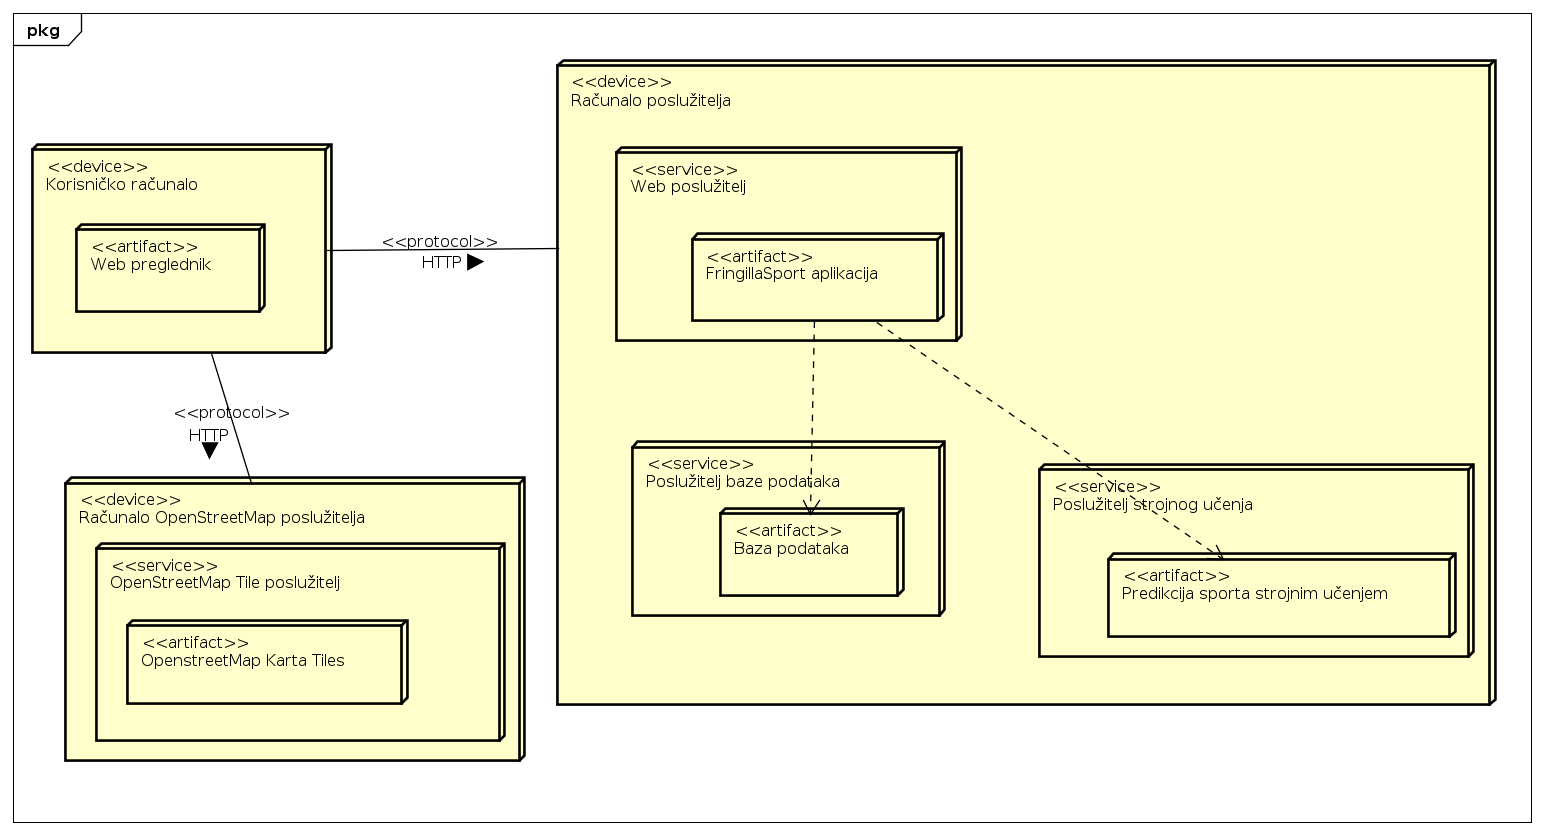
\includegraphics[width=\textwidth]{dijagrami/DeploymentDiagram0.png}
				 \caption{Dijagram razmještaja}
			\end{figure}
			
			\eject 
		
		\section{Upute za puštanje u pogon}
		
			Aplikacija je puštena u pogon na ubuntu 18.04 serveru. Te je na serveru potrebno imati instaliranu Javu 11.0, Node.js i Python 3.0.
			
			\subsection{Instalacija postgresql baze podataka}
			Potrebno je instalirati postgresql bazu podataka s naredbom:
			\begin{verbatim}
				$ sudo apt install postgresql postgresql-contrib
			\end{verbatim}
			Potom kreiramo bazu podataka za aplikaciju:
			\begin{verbatim}
				$ createdb-h localhost -p 5432 -U postgres fringilladb password pass
			\end{verbatim}
			Navedene podatke potrebno je unjesti u datoteku backenda na lokaciji backend/src/main/resources/application.properties:
			
			\begin{verbatim}
			spring.datasource.url=jdbc:postgresql://localhost:5432/fringilladb
			spring.datasource.username=postgres
			spring.datasource.password=pass
			spring.jpa.hibernate.dll-auto=create
			\end{verbatim}
			
			\subsection{Instalacija drugih potrebnih paketa}
			
			Za ostale komponente aplikacije potrebno je instalirati programe navedenim naredbama.
			
			\begin{verbatim}
				$ sudo apt install software-properties-common
				$ sudo apt install nodejs python3 python3-pip default-jre
			\end{verbatim}
		
			\subsection{Pokretanje backenda}
			Potrebno se je pozicionirati u direktorij izvorniKod/backend te pokrenuti naredbu:
			\begin{verbatim}
				$ ./mvn spring-boot:run
			\end{verbatim}
			
			\subsection{Pokretanje frontenda}
			Frontend aplikacije pokrece se pozicioniranjem u direktorij izvorniKod/frontend te izvršavanjem naredbi:
			
			\begin{verbatim}
				$ npm install
				$ npm start
			\end{verbatim}
			Prva naredba instalira potrebne pakete, dok druga pokreće frontend. 
			
			\subsection{Pokretanje servera za predlaganje sporta}

			Za pokretanje python servera potrebno se je pozicionirati u direktorij izvorniKod/mlSportPredict te pokrenuti naredbu:
			
			\begin{verbatim}
				$ python server.py
			\end{verbatim}
			
			
			Napomena zbog trenutne konfiguracije potrebno je stvoriti link između direktorija izvorniKod/backend/uploads i izvorniKod/frontend/public/documentation.
			
			\eject 
